%!TEX root = ../thesis.tex
\section{Evaluation}
To evaluate the DemoWiz design, we conducted a controlled experiment in which participants recorded and edited a demo video, and gave a presentation with the edited video. Specifically, we wanted to see if presenters would evaluate their own performances higher with the support of our augmented visualizations and control of timing.

\subsection{User Study}

\subsubsection{Baseline Condition: DemoWiz without Visualization}
Since DemoWiz allows for rapid editing of the video, it would have been unfair to compare it with a conventional video player without supporting any editing during the rehearsal phase. We therefore modified our system to serve as the baseline condition, providing participants with the same lightweight editing of the video in each condition. However, during presentation, the baseline condition was similar to a conventional video player that shows only the video without event timeline and augmented visualizations. It also did not support the \textit{stop} markers and \textit{text notes}, i.e., participants could only adjust playback speed of each segment and add variable length \textit{pauses}. During presentation, participants only saw the video with a traditional timeline. They could, however, pause (or stop) and resume the video manually at any time during playback.

\subsubsection{Study Design}
We conducted the study as a within-subjects design in a usability room. After recording and editing a video using the same system, each presenter gave a presentation with both systems to an experimenter. To control the effect of order and learning, we prepared two tasks that included similar interaction flows and counterbalanced the order of the two systems—DemoWiz and Baseline—but we fixed the order of tasks. Even though presenting to a single audience member in a usability room is not the same as using the system with a large conference audience, it is important to control the tasks and presentation as closely as possible to understand the relative benefits of the system in comparison with a baseline condition.

For each condition, we observed and coded the \textit{timing} of narration that matched the video content and noted the time in seconds when an event was described \textit{before}, \textit{at}, or \textit{after} the action happened in the demo video. We also marked obvious \textit{breaks} between narrations, \textit{errors} when the narration was not about the current or following events (e.g., discussing actions in a different order than they actually occurred), and \textit{misses} when an important action was not mentioned. To avoid unconscious bias that might influence the coding of the videos, we neutrally named the recordings and coded them all in a batch. We focused on objective timing measurements as much as possible, measuring deviation from specific video events and their corresponding narrations down to a second. Finally, we gathered qualitative feedback through satisfaction and preference questionnaires.

\subsubsection{Participants}
We recruited 12 participants (10 males and 2 females) from a software company. However, we excluded the data from two participants (1 male and 1 female); one was due to a software bug during one condition and another was because the participant requested to restart a presentation in one condition. The average age of the effective 10 participants was 37.3 ranging from 24 to 64 years of age. We recruited participants who had experience at showing a software demonstration to an audience such as giving a presentation at a conference. Four participants were native English speakers and the rest were fluent in English. The expertise of participants included audio processing, computer graphics, human-computer interactions, machine learning, networking, and software engineering. Each participant was compensated with lunch coupons worth \$20.

\subsubsection{Procedure and Tasks} Each session consisted of one training task and two experimental tasks. For the training task, to introduce the common features for recording and editing the video, we designed a simple workflow of five steps to demonstrate editing of a slide using PowerPoint. The experimenter briefly demonstrated an example and then introduced the recording program that captured the screen. Participants were then asked to practice and record using the recording program.

The two tasks consisted of a similar sequence and interactions: 1) searching with Bing Maps to show the 2D map view and the Bird's Eye view, looking for a restaurant, and navigating to the interior view of a specific restaurant; and 2) searching with Google Shopping to show the search results with the Grid view, filtering and voting for reviews, and navigating the 3D product view of an espresso machine. For each task, we provided a specific scenario along with a list of subtasks. The experimenter walked through this list with participants to ensure that they could easily find the features that needed to be demonstrated. Participants were then asked to practice (3-5 minutes), record (about 2 minutes), and rehearse and edit (5-10 minutes).

To help simulate a conference setting where participants would not be able to present immediately after having recorded a demonstration, we inserted an intentional 1-minute gap between rehearsal and presentation. During this gap before giving the presentation, we asked participants to watch a conference showcase video. Participants were then asked to stand up and gave a 2-3 minute presentation to the experimenter in a usability room.

After each task, participants filled out a questionnaire of 8-10 questions asking about their experience (8 for the Baseline condition, and 10 for the DemoWiz condition). At the end of the session, an online questionnaire was provided for them to present overall preferences and leave comments. Each session lasted about 1.5 hours.

\subsubsection{Experiment Setup}
Each participant used a desktop computer running Windows 7, Expression Encoder 4 for screen recording, and a web browser for the DemoWiz user interface. A regular mouse and keyboard were provided, along with two 27-inch displays, one for editing (during rehearsal) and showing the audience view (during presentation, see Figure~\ref{fig:demowiz_results_two_views} right), and the other for the presenter view (see Figure~\ref{fig:demowiz_results_two_views} left) on a stand-up table. The resolution of both displays was 1920×1200 pixels. The average captured screen area was 1311×857 pixels. In the presenter view, the video resolution was within 1000×600 pixels; in the audience view, the screencast videos were resized to fill the entire display with at least 100-pixel wide border in black. During the study, the experimenter stayed in the room, providing instructions and sitting behind the participants during the recording and editing phases.

\begin{figure}
  \centering
  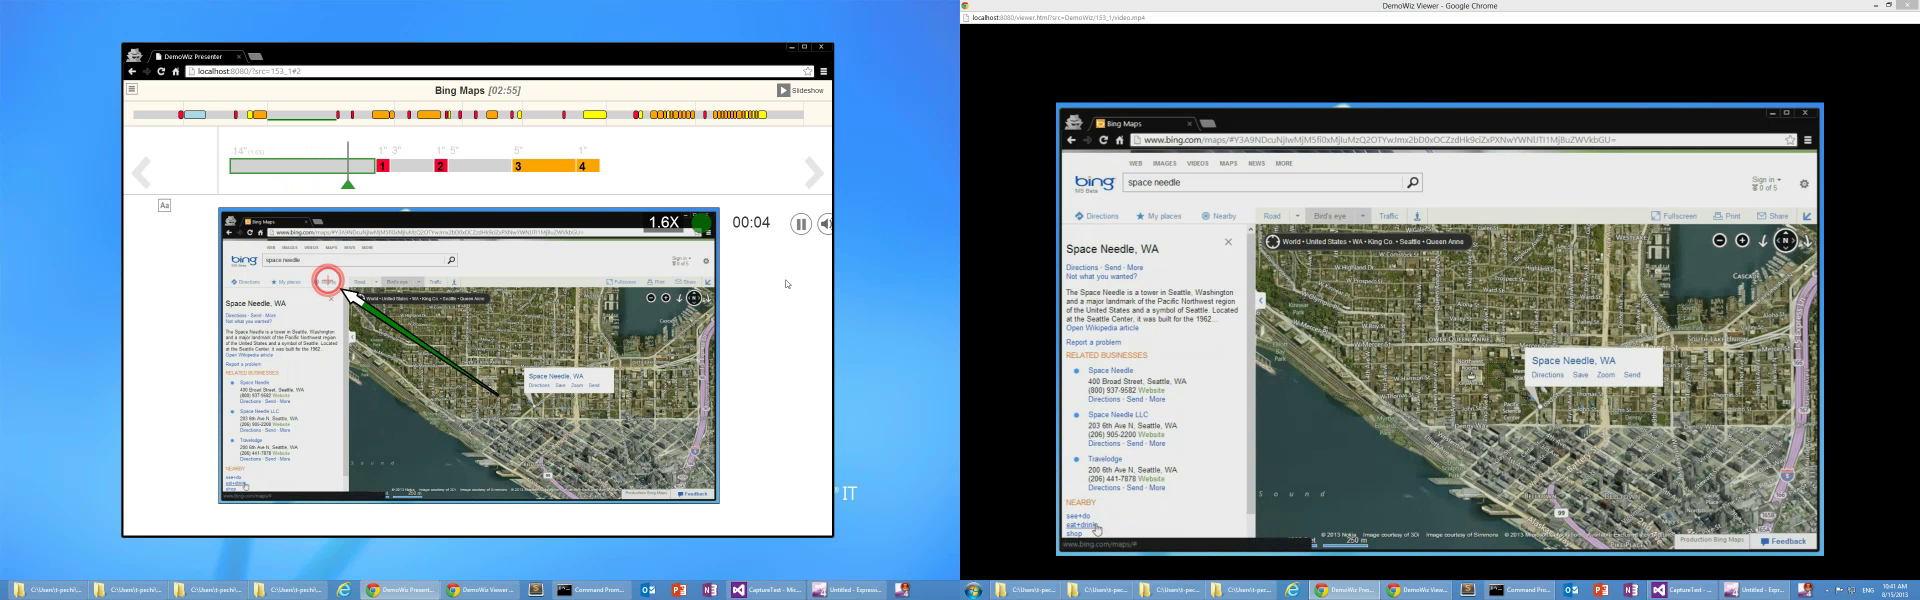
\includegraphics[width=\columnwidth]{\demowiz/fig/study_result}
  \caption{Participants saw the presenter view, shown on the left, while giving a presentation in the study. The audience view on the right was shown in the other display at the same time.}
  \label{fig:demowiz_results_two_views}
\end{figure}

% ---------------------------------------------------------------

\subsection{Results}
Ten participants successfully recorded, rehearsed, and gave a demo with both systems.

\subsubsection{Subjective Preference}
Figure~\ref{fig:demowiz_likert} shows the average subject responses (on the 7-point Likert scale) from presenters for both systems. We analyzed these subjective responses using a Wilcoxon signed-rank test. We found significant differences in responses for ease of narration (DemoWiz µ = 6.2 over Baseline µ = 4.5, \textit{p} = .018) and ease of presentation (6.4 over 5.2, \textit{p} = .048). We also found marginally significant differences in participants' overall satisfaction with their presentations (5.5 over 4.7, \textit{p} = .062). Participants also tend to agree that DemoWiz helped them interpret timing (6.1 over 4.4, \textit{p} = .067).

In addition, 9 out of the 10 participants preferred DemoWiz to the system without visualization and would choose to present with DemoWiz if they were asked to give a public software demo; the remaining participant indicated no preference for both questions. The general feedback was also encouraging. For example, P1 commented \iquote{Awesome system. I'd use it today.} and P5 \iquote{felt more confident in being able to present what I wanted to.}

\begin{figure*}[t]
  \centering
  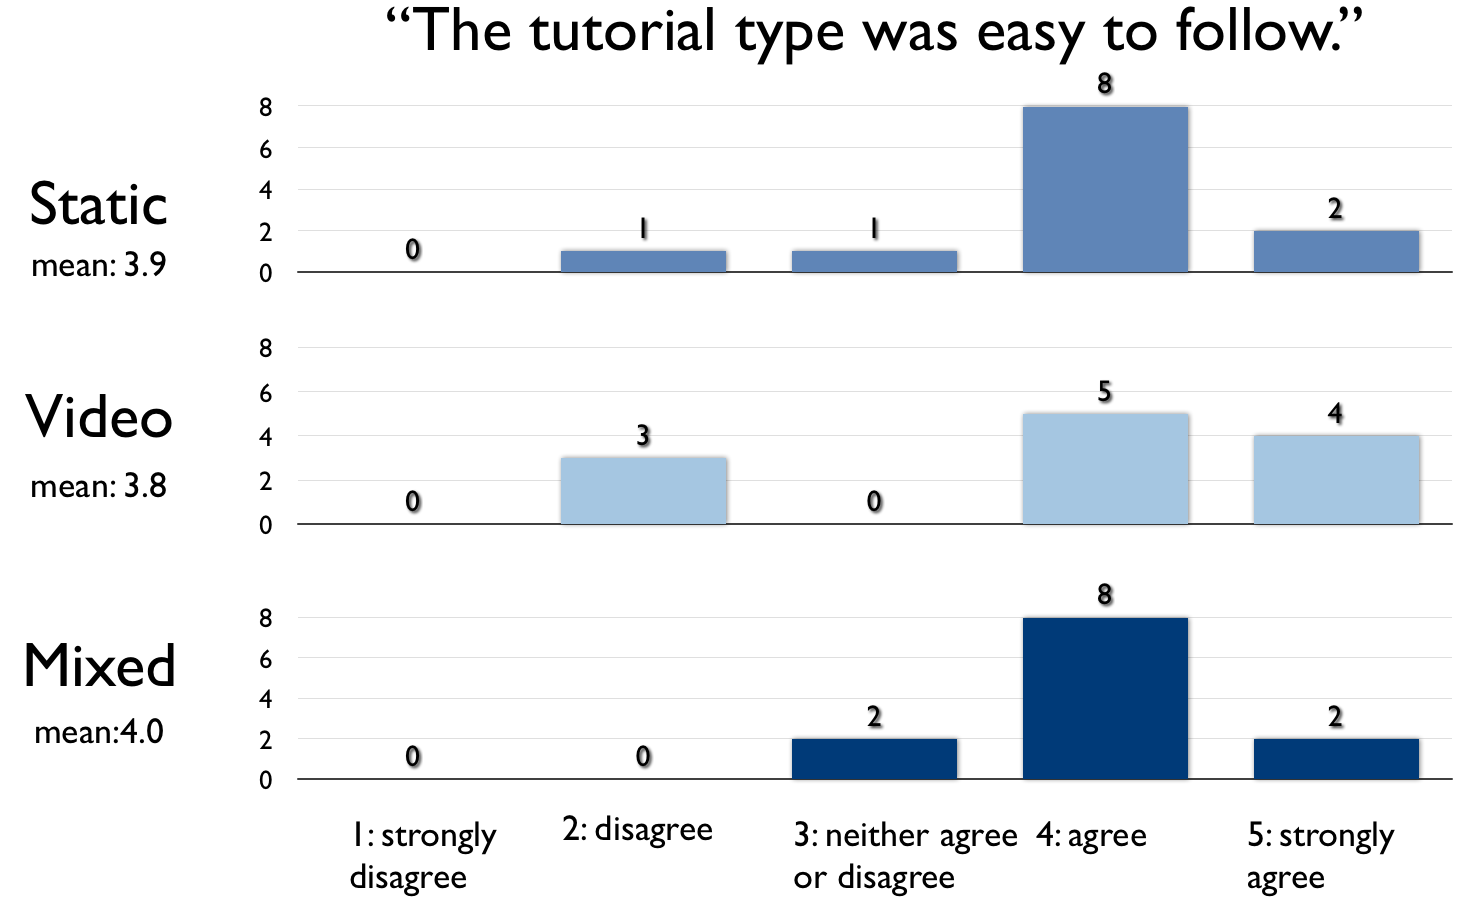
\includegraphics[width=0.6\textwidth]{\demowiz/fig/results/likert}
  \caption{User feedback from questionnaire on the 7-point Likert scale.}
  \label{fig:demowiz_likert}
\end{figure*}

\subsubsection{Visualization as a Supportive Cue}
Participants answered that they were able to understand DemoWiz visualization of input events (µ = 6.0) and found it supportive for their presentations (µ = 6.3). They also commented that the DemoWiz visualization supported the presentation in various aspects: \iquote{the visualization reminds of the order of the content} (P1), \iquote{Really liked the ability to know what was coming up} (P2), \iquote{It provides better insight of the progress of the video} (P6), and \iquote{viz gave me an idea about timing or something I was going to forget to say} (P9).

\subsubsection{Narration Timing}
We coded the 20 recordings of participants' final presentations to observe the timing of narration of each action in correspondence with the video content (11 key events for both tasks). With DemoWiz, participants tended to \textit{anticipate} the upcoming events rather than talk afterwards, where the average timing was -0.1 seconds with DemoWiz (i.e., narrated the action before it happened) and 0.4 seconds with the Baseline condition (i.e., explained the action after it was shown). We found a significant difference in the number of times that events were anticipated by the narration, co-occurred, or occurred after the fact ($\chi $\textsuperscript{2}\textit{(2,220) = 8.6, p = .01}, see Figure~\ref{fig:demowiz_results_timing}).

In general, this supports our suspicion that DemoWiz would help in anticipating an event as opposed to talking about it after it occurred. More important though, was how often a narrator spoke about an event within several seconds of when the event actually occurred. By defining \textit{better} timing as when a presenter's explanation came within 2 seconds of a shown event (either prior, exact, or after), there was marginal significance by condition (\textit{p} = .089 with DemoWiz performing better). In addition, with the Baseline condition, the timing of narration was less consistent and off more, varying from 6 seconds early or 10 seconds late with a variance of 3.9 seconds, in comparison to the DemoWiz condition with at most 3 seconds early to 3 seconds late and a variance of 1.9 seconds.

Five participants had an obvious \textit{error} (forgot the next action or incorrectly narrated another action), had a long \textit{break} (waiting for more than 2 seconds until the action was made), or \textit{missed} an action (did not explain an important feature) when presenting with the Baseline condition. On the other hand, in the DemoWiz condition no errors were made, and there were only one long break and one miss from two different participants, respectively.

Participants' comments also support the fact that DemoWiz helped presenters anticipate the upcoming events. P7 explained, \iquote{(I) felt better able to time my speech to coincide with visual events, rather than trailing after them. Without the event visualizations, I felt like I was talking about what the audience had just seen, rather than having my words and visuals combine to a single message.}

\begin{figure*}[t]
  \centering
  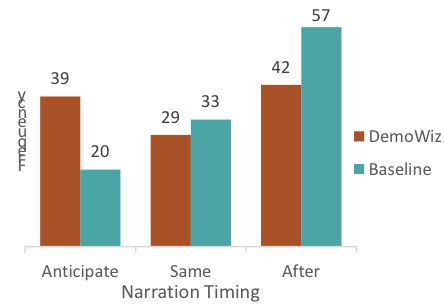
\includegraphics[width=0.5\textwidth]{\demowiz/fig/results_timing}
  \caption{The number of times events were anticipated by the narration, co-occurred, or occurred after the fact.}
  \label{fig:demowiz_results_timing}
\end{figure*}

\subsubsection{Editing Experience}
We collected comments on the workflow. Participants found it easy to record (µ = 6.4) their demonstrations with DemoWiz. For editing features, they found it easy to edit in general (6.6), including controlling the playback speed (6.5) and adding pauses and stops (6.5), but it was less easy to add text notes (4.8); only two participants used this as reminders.

Although using different strategies, all of the participants adjusted the playback speed for matching their narration. Some sped up whenever possible and added stop markers for transitions; some slowed down the repetitive actions (such as drags) to demonstrate effects. P6 said, \iquote{I really liked being able to add `stop' events so I could `fake' my demo better.} DemoWiz made it easy for participants to separate the capturing and presentation preparation as P5 explained, \iquote{Overall, recording was very easy. In fact, as I got to the second task, I realized that I really don't need to think about the words as I record because later on I will be able to slow down and speed up time ...}

On average, the length of demo videos was 2'09'' before editing and 2'05'' after editing, and the presentation was 2'38'' long. Each participant spent 7.5 minutes on average to edit. For each demo of 44 segments on average, participants adjusted 3.15 segments for speedup and 4.25 segments for slowdown, and added 0.55 pause markers. In the DemoWiz condition, 1.2 stop markers and 0.2 text notes were added.
